\documentclass{article}
\usepackage[utf8]{inputenc}
\usepackage[a4paper, total={6in, 8in}]{geometry}
\usepackage{graphicx}

\title{CMSC426Pj2 Report}
\author{Yizhan Ao UID: 116022064}
\author{
  Yingqiao, Gou\\
  \texttt{ygou@terpmail.umd.edu}\\
  \texttt{UID:115979000}
  \and
  Yizhan, Ao\\
  \texttt{josephao@umd.edu}\\
  \texttt{UID:116022064}
  \and
  Daniel, Song\\
  \texttt{@umd.edu}\\
  \texttt{UID:}
}

\date{October 20 2021}

\begin{document}




\maketitle

\section{Introduction}
\begin{enumerate}
   \item 
\end{enumerate}

\section{ANMS: 25 pts}
The goal of ANMS is to pick out the stronger corner points.\\
\begin{itemize}
    \item Using the cornermetric method to find all the corners of each grayscale image. 
    \item After applying imreagionalmax, we can get the strong corners in the image.
    \item Using ANMS alogrithm we can find the best pixel of each image.
    \item We analyze a 40*40 pixel square area selecting an intial 300 N-best to trial.
    \item Note: Each image may vary from sizes
\end{itemize}
\textbf{Shortcoming} 
\begin{itemize}
    \item We specify the N-best manually choosing from 450 - 300 - 200- 100 -50
    \item The problem we think is that the level of the variable is affecting to understand the sets
    \item Even though the variable is performed well in terms of the point indication, however, we think the point may be not accurate in some points
    \item ANMS takes the amount of points which are equally distributed. However, removing some of better score points in a high score area will resulted in less accurate data in dense areas. 
    \item This could resulted to a decrease in accuracy in the feature matching and warping.

\end{itemize}

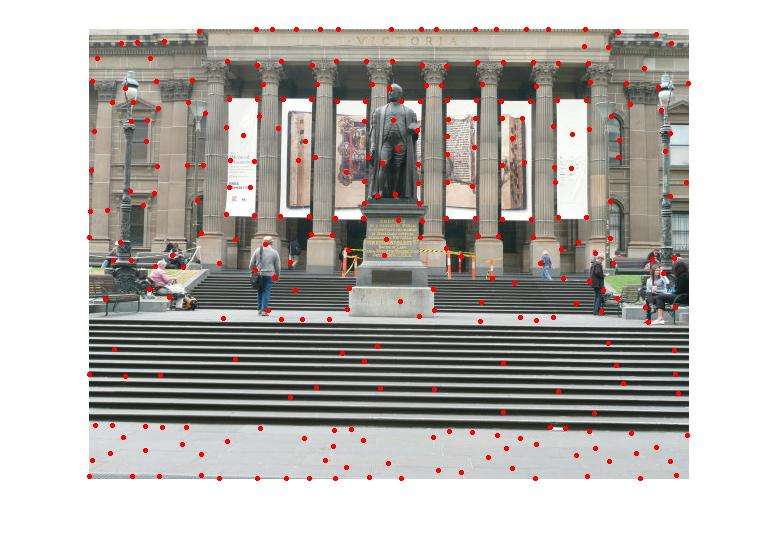
\includegraphics[scale = 0.5]{anms1.jpg}\\
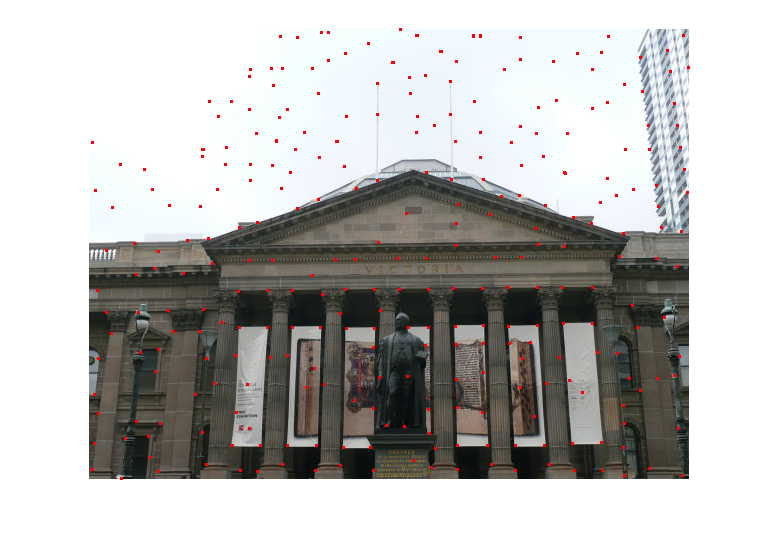
\includegraphics[scale = 0.7]{anms2.png}\\
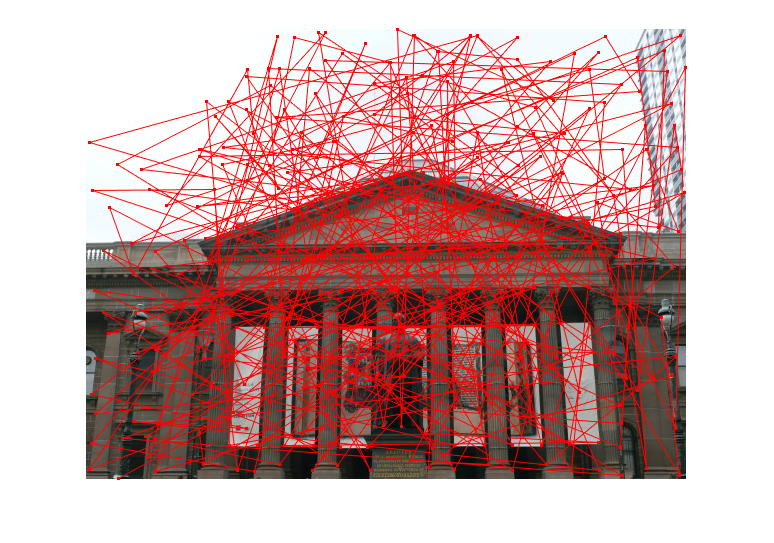
\includegraphics[scale = 0.5]{ANMS4.png}\\
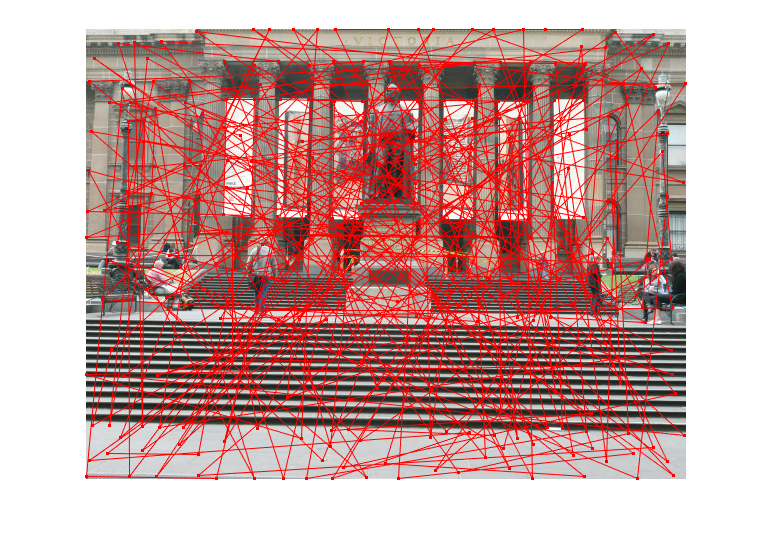
\includegraphics[scale = 0.7]{ANMS5.png}

\section{Feature Descriptors: 15pts}

\section{Feature Matching: 15pts}

\section{RANSAC and Homography Estimation: 20pts}
 
 
 
\section{Image Warping (and Blending): 25pts}

\section{Panoramas}


\section{Conclusion}




\begin{itemize}

    \item ANMS: 25 pts
    \item Feature Descriptors:15pts
    \item Feature Matching: 15pts
    \item RANSAC and Homography Estimation: 20pts
    \item Image Warping (and Blending): 25pts

\end{itemize}
\end{document}



